% 公立はこだて未来大学 卒業論文 テンプレート ver1.50
% (c) Junichi Akita (akita@fun.ac.jp), 2003.10.31
% update by N.T.,  2004.11.10
%
\documentclass{funthesis}
%\documentclass[english]{funthesis} % use [english] option for English style

\usepackage{graphicx} % 図(EPS形式)を本文中で読み込む場合はこれを宣言
\usepackage{url}

% この部分に,タイトル・氏名などを書く.
% タイトルなどの定義の始まり
\jtitle{移動手段・時間を考慮した旅のしおりによる\\
観光スケジュール作成支援 }  % 論文の和文タイトル
%
\etitle{Support for Making Tourism Schedule for Traveler's Notebook that Considered Moving Transportation and Time
}% 論文の英文タイトル
%
\htitle{Support for Making Tourism Schedule}   % ヘッダー用の論文の短縮英文タイトル
%     必ず1行に収まるように英文タイトルを短縮する.
%
\jauthor{辻浦 崇大}     % 氏名(日本語)
\eauthor{Takahiro Tsujiura}   % 氏名(英語)
\jaffiliciation{情報アーキテクチャ学科} % 所属学科名(日本語)
\eaffiliciation{Department of Media Architecture} % 所属学科名(英語)
\studentnumber{1012178}   % 学籍番号
\jadvisor{伊藤 恵}    % 正指導教員名(日本語)
%\jcoadvisor{副指導 教員} % 副指導教員(日本語)がいる場合は
                        % コメントアウトし名前を書く
                        % 副指導教員がいない場合は,ここは削除しても可
\eadvisor{Kei Ito}  % 正指導教員名(英語)
%\ecoadvisor{Prof. Coadvisor}   % 副指導教員(英語)がいる場合は
                         % コメントアウトし名前を書く
                         % 副指導教員がいない場合は,ここは削除しても可
\jdate{平成28年1月29日}    % 論文提出日   (日本語)
\edate{January 29, 2016}     % 論文提出年月 (英語)
% タイトルなどの定義の終わり

\begin{document}

%--------------------------------------------------------------------
\maketitle       % タイトルページを作成

%--------------------------------------------------------------------
% 英文概要(250語程度)
\begin{eabstract}
This study tries to make Traveler's Notebook that considered moving transportation and time for making tourism schedule efficiently.
Making individual travelers tourism schedule are difficult.
It's reasons are three. First, they are difficult to grasp moving transportation and time. Second, they need to search information from many locations that needs travel. Third,  they are difficult to understand visually.
Making Traveler's Notebook tools as one of the means facilitate them.
But existing Traveler's Notebook tools almost entering tourist attraction, moving transportation and time manually.
I think that making tourism schedule efficiently is possible not only displaying destination but also include Traveler's Notebook moving transportation and time between destination and destination.
This study consider fun in trip, after trip 
and tries to support the combination of existing tools displaying destination, adding the lists moving transportation and time and individual travelers have fun more.

\end{eabstract}

% 英文キーワード(5個程度をコンマ(,)で区切って羅列する)
\begin{ekeyword}
Keyrods1, Keyword2, Keyword3, Keyword4, Keyword5
\end{ekeyword}

%--------------------------------------------------------------------
% 和文概要(400字程度)
\begin{jabstract}
効率的な観光スケジュール作成を支援するために,移動手段・時間を考慮した旅のしおりの作成を試みる.
個人旅行者が観光スケジュールを作成することは難しい.
その理由として移動手段・時間を把握しにくいということ,旅行に必要な情報を様々な場所から探す必要があること,視覚的にわかりやすく作成しにくい,などが挙げられる.
それらを行いやすくするための手段の1つとして,旅のしおり作成ツールが存在する.
しかし既存の旅のしおり作成ツールは移動手段・時間を考慮せず,観光スポットや移動手段・時間を手動で入力するものが多い.
そこで目的地を表示するだけでなく,目的地間の移動手段・時間を旅のしおりに組み込むことで効率的な観光スケジュール作成の支援が可能になると考えた.
また旅行計画中や旅行後の振り返り時の楽しさも考慮する.
本研究では既存のツールを組み合わせることで目的地を表示すること,目的地間の移動手段・時間を目的地のリストに加えることの他,旅行をより楽しむことの支援を試みる.

\end{jabstract}

% 和文キーワード(5個程度をコンマ(,)で区切って羅列する)
\begin{jkeyword}
観光, 旅のしおり, ああああ, キーワード4, キーワード5
\end{jkeyword}

%--------------------------------------------------------------------
\tableofcontents % 目次を作成


% 本文のはじまり
%--------------------------------------------------------------------
\chapter{序論} % 1章のタイトル
%\chapter{Introduction} % sample of English style

123456789012345678901234567890
123456789012345678901234567890
123456789012345678901234567890
123456789012345678901234567890
123456789012345678901234567890

123456789012345678901234567890
123456789012345678901234567890
123456789012345678901234567890
123456789012345678901234567890
123456789012345678901234567890

% \includegraphics[width=??cm]{hoge.eps} % 図(EPS形式)を読み込む場合

\section{背景} % sectionのタイトル

% 以下に背景,関連する環境,状況,技術に関する概要を記述.

手続き型言語では,巨大システムを構築し,管理を行うことが難しいため,こ
こにオブジェクト指向という新たな考え方を導入して新しいプログラミング言
語を作成することにした.

\section{対象とする領域}

実用レベルのサイズのプログラムを作成するためのプログラミング言語につい
て研究する.ここで,行うのは3次元グラフィックス向けの言語の設計とその
インタプリタの実装である.

\section{研究目標}

完全な処理系の実装を目指すものではなく,プログラミング言語にオブジェク
ト指向という考え方を取り入れたプログラミング言語を設計し,プロトタイプ
システムを作成することにより,オブジェクト指向の概念が,プログラミング
の能率向上とメンテナンス性の向上に寄与することを示す.

%--------------------------------------------------------------------
\chapter{関連研究}% 2章のタイトル

\section{CT-Planner}

%\subsection{Smalltalk-80} % subsectionのタイトル

本研究の関連研究としてWebサービスによる対話型の旅行計画支援ツール「CT-Planner」[1]がある.
このツールは不慣れな土地での旅行計画作成に不安を抱く個人旅行者を対象としたものであり,函館や横浜などの都市を選択し「のんびり歩こう」「文化を知りたい」等の旅行スタイルの中から自分の嗜好に合ったものを選択すると,選択した旅行スタイルに応じた観光スポットを巡る旅行プランが自動的に作成される.旅行プラン作成後もユーザは行きたい観光スポットを適宜変更でき「穴場好き」か「有名所好き」等の特性を選ぶことでユーザの嗜好に合った旅行プランに変更できる.

%\subsubsection{必要があれば} % subsubsectionのタイトル
% ※ subsubsectionはあまり使わないほうがよい

.


%--------------------------------------------------------------------
\chapter{研究のアプローチ}% 3章のタイトル

本研究では始めに既存の旅のしおりの利点,問題点の調査を行った.次に旅行計画の作成についての考え方を知るために旅行計画作成に関するアンケートを行った.また,ツールを作成するうえで必要になる機能を調査するために予備実験を行う.その後,作成するツールの設計・実装を行う.

\section{提案する言語FUNの特徴}

この言語の特徴は,..であり,...という従来にない長所をもつ.

\section{言語仕様}

言語仕様は以下の通り.


\section{実装方法}

この言語は,C言語を用いて記述されている.ソースコードは20に分かれ,
コードの大きさは約3000行となった.

\subsection{開発環境}

この言語は,C言語を用いて記述されている.ソースコードは20に分かれ,
コードの大きさは約3000行となった.

\subsection{OSに対する依存性}

この言語は,C言語を用いて記述されている.ソースコードは20に分かれ,
コードの大きさは約3000行となった.


%--------------------------------------------------------------------
\chapter{調査}% 4章のタイトル

\section{既存の旅のしおり作成ツールの調査}

既存の旅のしおりは大きく分けて「観光スケジュールを作ることに重点を置いたツール」と「旅のしおりを作ることに重点を置いたツール」が存在する.\\
 1つ目の「観光スケジュールを作ることに重点を置いたツール」とは観光スポットや飲食店等をツールの内で検索し,自分の行きたい観光スポット等をスケジュールに組み込んで作っていくというものである.この例として「ポケたび」[2]という旅行の計画を「旅のしおり」として作成・保存することができるツールがある.このツールでは旅行したい場所をエリアから選ぶまたは検索することで指定し,移動時間や滞在ホテルを指定することができる.また,このツールでは移動手段・時間は手動で入力する.\\
 2つ目の「旅のしおりを作ることに重点を置いたツール」とは印刷すると修学旅行等で作るような冊子のしおりになるものである.こちらはしおりの外面のデザインや写真といったことも決められるツールが多い.この例として「旅のしおり工房」[3]という旅計画をたて「自分だけのガイドブック」をしおりにして持っていくことができるツールがある.このツールは始めに表紙の画像やデザインを決め、次に旅のテーマ,日程表などを作成していくことで冊子のしおりのように作ることができる.また,このツールでは旅行予定の場所や移動手段・時間は手動で入力する.\\
 上記の2つのツールを「観光スケジュールが作成できるか」「観光スポットが検索できるか」「移動手段・時間が表示されるか」「しおりのデザインが決定できるか」の4つの観点で比較した場合,表1のようになる.

\begin{table}[htb]
\begin{center}
\caption{既存の旅のしおり作成ツールの比較}
  \begin{tabular}{|c|p{2.4cm}|p{2.4cm}|p{2.4cm}|p{2.4cm}|} \hline
     & 観光スケジュールの作成 & 観光スポットの検索 & 移動手段・時間の表示 & しおりのデザインの決定 \\ \hline 
    ポケ旅 & ○ & ○ & ○ & × \\ \hline
    旅のしおり工房 & ○ & × & × & ○ \\ \hline
  \end{tabular}
  \end{center}
\end{table}


この調査からこれらの旅のしおり作成ツールでは移動手段・時間を表示していないということがわかった.\\



\subsection{旅行計画作成に関するアンケート}
次に本学の学生,教員,事務員に対して旅行計画作成に関するアンケートを行った.52人にアンケートの回答を依頼したところ18人から回答があった.\\
 「旅行前に旅行の計画を紙やファイルなどをどこかに記録するか」という質問に対して「計画を立てて記録する」が56\%,「計画を立てるが記録しない」が33\%,計画を立てないが11\%であった(図1).「計画を立てて記録する」と回答した人は具体的に紙やGoogleドライブに記録するという回答があった.
\begin{figure}[htpb]
\begin{center}
%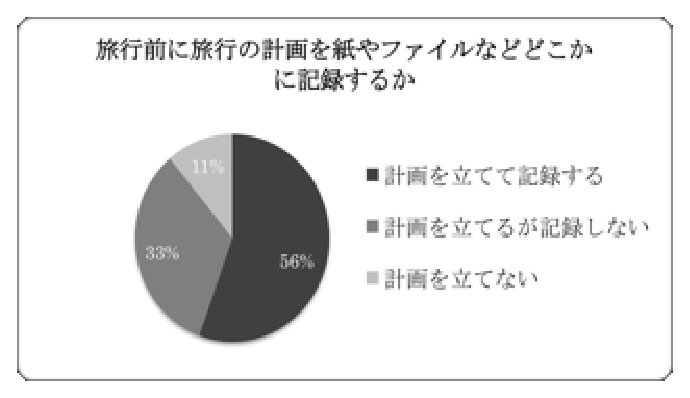
\includegraphics[width=4cm, height=2cm]{filerecord.eps}
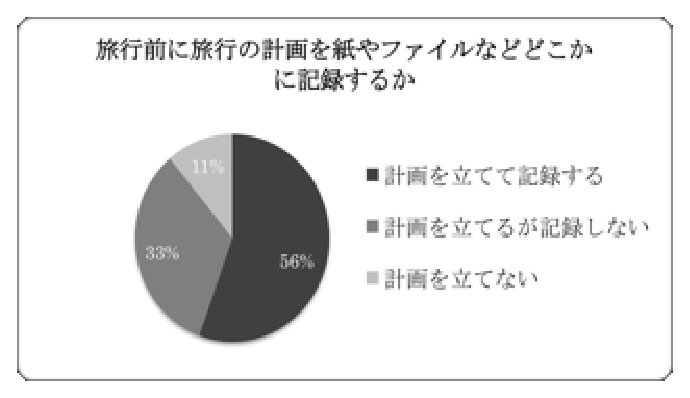
\includegraphics[scale=1.0]{filerecord.eps}
\caption{旅行前に計画を記録するか}
\end{center}
\end{figure}

「旅行前に旅行の計画を誰かに話すか」という質問に対して「はい」は84\%「いいえ」は11\%「旅行の計画を立てない」が5\%であった(図2).\\
\begin{figure}[htpb]
\begin{center}
%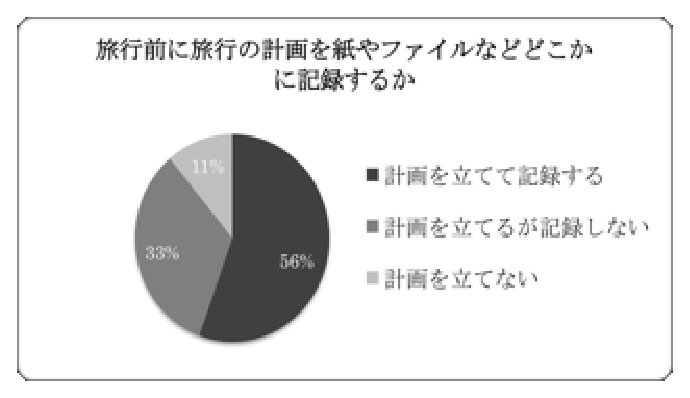
\includegraphics[width=4cm, height=2cm]{filerecord.eps}
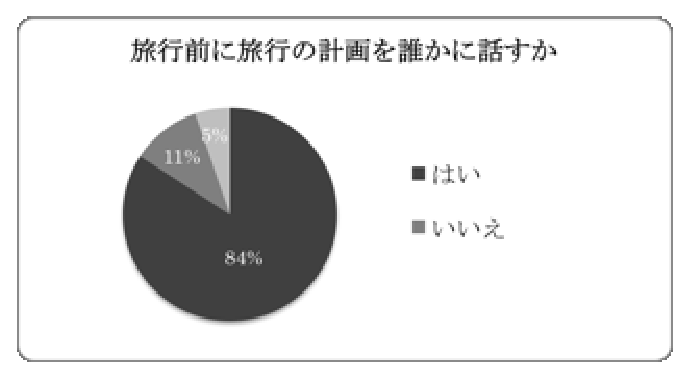
\includegraphics[scale=1.0]{beforetalktrip.eps}
\caption{旅行前に計画を話すか}
\end{center}
\end{figure}

「旅行後に旅行の計画を誰かに話すか」という質問に対して「はい」は32\%「いいえ」は63\%「旅行の計画を立てない」が5\%であった(図3).\\
\begin{figure}[htpb]
\begin{center}
%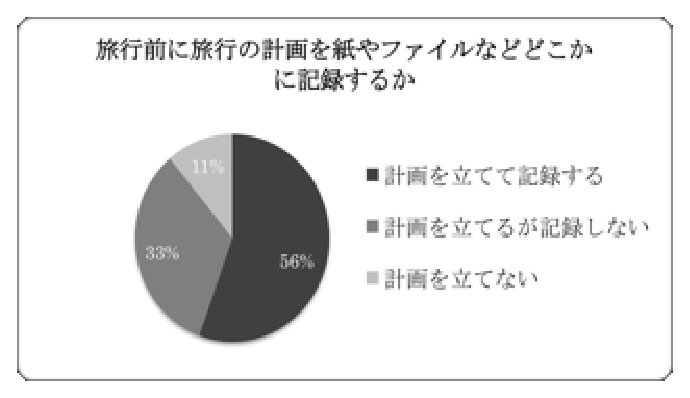
\includegraphics[width=4cm, height=2cm]{filerecord.eps}
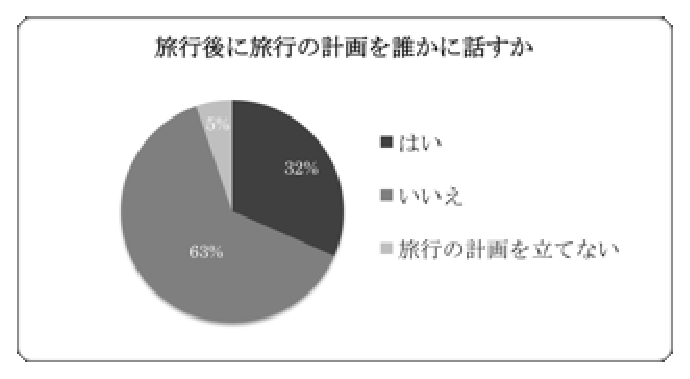
\includegraphics[scale=1.0]{aftertalktrip.eps}
\caption{旅行後に計画を話すか}
\end{center}
\end{figure}

「旅行の計画を立てることをどう思うか(複数回答可)」という質問に対して,「楽しい」という回答が最も多く次点で「面倒」「わくわくする」「自分で立てたい」が続いた(図4).\\
\begin{figure}[htpb]
\begin{center}
%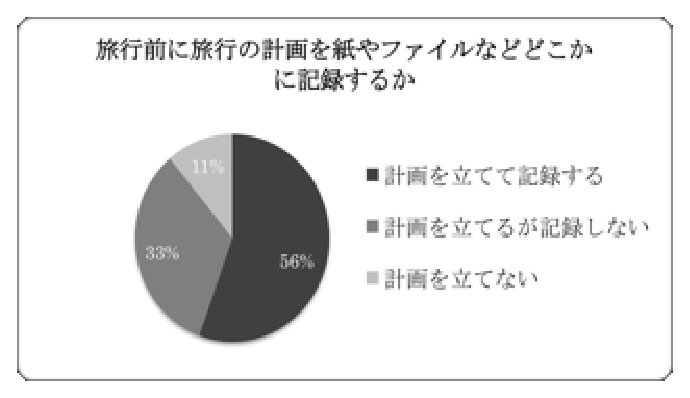
\includegraphics[width=4cm, height=2cm]{filerecord.eps}
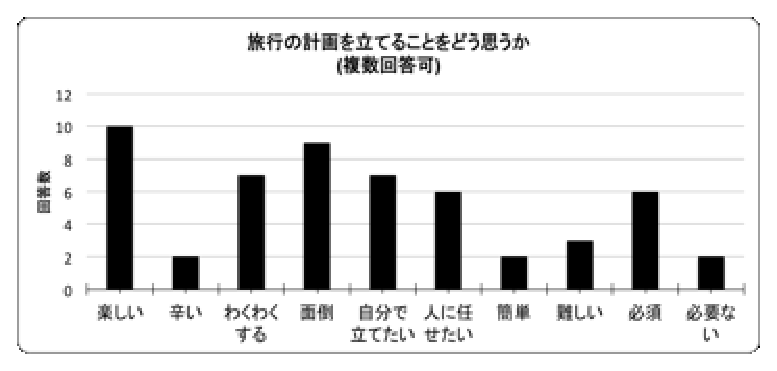
\includegraphics[scale=1.0]{howthinktrip.eps}
\caption{旅行計画を立てることをどう思うか}
\end{center}
\end{figure}

これらの結果から,旅行の計画を立てる人は多く,旅行前に計画を話すということも行われることが多いとわかった.また,旅行計画を立てることに楽しさを感じる人が多いが,面倒だと感じる人も多い.そのためツールで楽しさを感じてもらいつつ,面倒さを解消することが必要になる.\\



%--------------------------------------------------------------------
\chapter{予備実験}% 5章のタイトル

ツールを作成するうえで必要になる機能,特に「楽しさ」という観点で見た場合にどのような要素が必要になるかということや,どのような場面でユーザは「楽しさ」を感じているかということを調べるために予備実験を行う.この予備実験を計画する際に本学の認知科学に詳しい教員にアドバイスをいただいた.その内容は「被験者は1名ではなく2名で行ってもらい,その2名も可能であれば実際に旅行に行くような間柄の関係の人にすべき」,「複数の案から選択できるような形式にする」,「被験者の発言内容,表情,口調などから読み取れることがある」というものであった.そこで予備実験の方法として,被験者2名ずつペアになってもらい,こちらが数パターン用意した旅行計画の概要の中から行きたいというものを選んでもらう.また既存のツールを用いて実際に旅行計画を立ててもらうということを考えている(図5).
\begin{figure}[htpb]
\begin{center}
%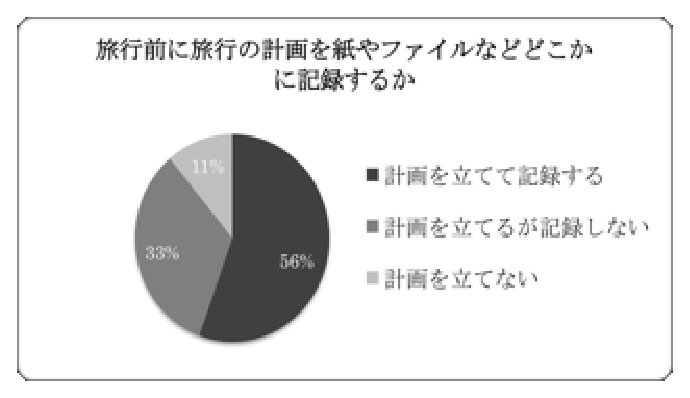
\includegraphics[width=4cm, height=2cm]{filerecord.eps}
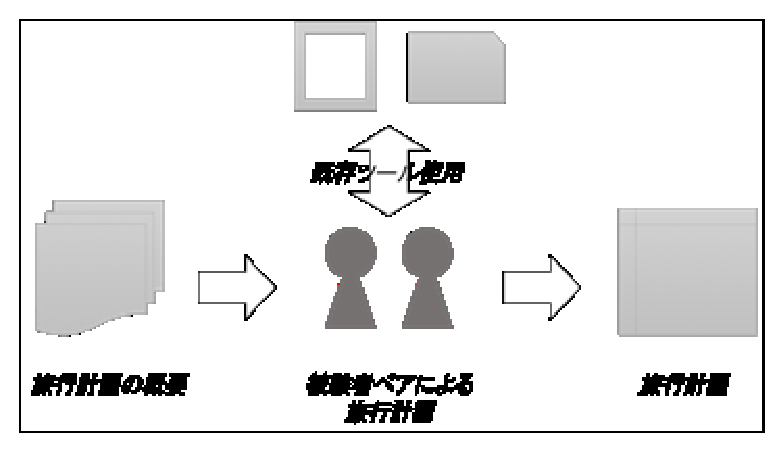
\includegraphics[scale=0.65]{semiexp.eps}
\caption{予備実験イメージ}
\end{center}
\end{figure}

この際,被験者には思考の過程を声に出しながら行ってもらうことで,より被験者の思考がわかりやすくしたいと考えている.また被験者の表情や発話の内容,などを記録し分析する.\\

\section{評価結果}

Java言語との比較では,惨敗であり,FUNは2倍の
記述量を必要とした.しかし,これは,Javaのもつ
パッケージIKURAが非常に強力であるためで,
同一機能をもつライブラリを用意することにより,
FUNにも同様の能力を持たせることができることが判明した.

\section{評価結果}

Java言語との比較では,惨敗であり,FUNは2倍の
記述量を必要とした.しかし,これは,Javaのもつ
パッケージIKURAが非常に強力であるためで,
同一機能をもつライブラリを用意することにより,
FUNにも同様の能力を持たせることができることが判明した.

%--------------------------------------------------------------------
\chapter{作成するツール}% 6章のタイトル

現時点ではツールの構成イメージとしてAPI等を用いて地図や乗り換え案内,ルート検索などのツールと組み合わせ移動手段・時間を表示する(図6).
\begin{figure}[htpb]
\begin{center}
%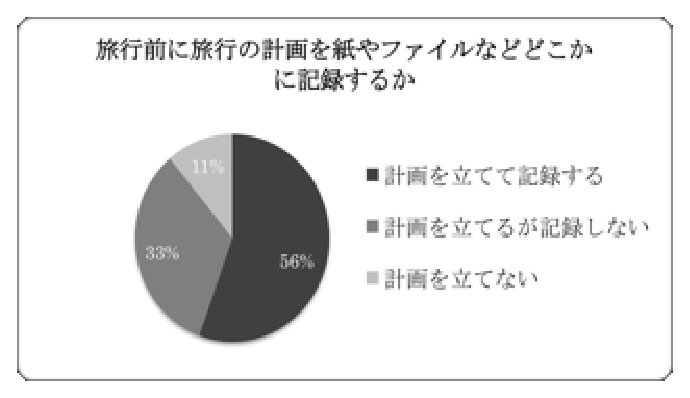
\includegraphics[width=4cm, height=2cm]{filerecord.eps}
\includegraphics[scale=0.3]{willmaketools2.eps}
\caption{作成ツールイメージ}
\end{center}
\end{figure}

詳細は未定だがツール作成において「楽しさ」を感じることができるように工夫する.どのような要素が満たされていると旅行計画に「楽しさ」を感じてもらえるかは予備実験の結果を参考にする.\\

%--------------------------------------------------------------------
\chapter{結論と今後の展開}% 7章のタイトル

\section{まとめ}

本研究ではツールを組み合わせ,移動手段・時間を考慮した旅のしおりによる観光スケジュール支援を行う.現段階では既存のツールと旅行計画作成の考え方の調査を行い,既存の旅のしおり作成ツールは移動手段・時間を考慮していないこと,旅行計画を立てる人の割合が多いこと,旅行計画作成について「楽しい」「面倒」と考える人が多いことがわかった.\\
 今後はユーザが旅のしおりを作成するうえで「楽しさ」を感じてもらうためにはどのようなことが必要になるかということや,そのことを踏まえて必要機能の検討とツールの設計,実装を行う.



\section{今後の方針}

Java言語との比較では,惨敗であり,FUNは2倍の
記述量を必要とした.しかし,これは,Javaのもつ
パッケージIKURAが非常に強力であるためで,
同一機能をもつライブラリを用意することにより,
FUNにも同様の能力を持たせることができることが判明した.


%--------------------------------------------------------------------
%\chapter*{謝辞}



%--------------------------------------------------------------------
% 参考文献
\begin{thebibliography}{9}
 \bibitem{blgen} 倉田陽平ら,旅行プラン作成ツールCT-Plannerのプラットフォーム化に向けて,観光情報学会第11回全国大会,pp.38-39,2014
\bibitem{webp}  {\url{https://poketabi.com/}}
\bibitem{wagby}  {\url{https://www.mapfan.com/shiori/}}
\end{thebibliography}


% 以降,付録(付属資料)であることを示す
\appendix

%--------------------------------------------------------------------
\chapter*{付録その1} % \chapter{}を使うと「付録A ***」となる

付録その1(プログラムのソースリストなど)を必要があれば載せる

%--------------------------------------------------------------------
\chapter*{付録その2}

付録その2(関連資料など)を必要があれば載せる

%--------------------------------------------------------------------
% 図一覧
\listoffigures

%--------------------------------------------------------------------
% 表一覧
\listoftables

\end{document}
